%%
%%  chapter06.tex - Obstacle Detection and Planning for Autonomous Vehicles based on Computer Vision Techniques
%%
%%  Copyright 2014 Néstor Morales <nestor@isaatc.ull.es>
%%
%%  This work is licensed under a Creative Commons Attribution 4.0 International License.
%%

\graphicspath{{./images/chapter06/bmps/}{./images/chapter06/vects/}{./images/chapter06/}}

\chapter{Global Planning}\label{ch:chapter06}

Until now, we have seen several methods whose goal is the detection and, eventually, the tracking of objects in the surrounds of our prototype. However, at this point, we are not doing anything to avoid them. We need an strategy that allows an intelligent response when an obstacle is found, while allowing reaching a given point in the map efficiently. For this purpose, we need a set of planning algorithms that, given a map, localization information and information about the surrounding obstacles, allow doing these tasks. This set of algorithms is divided in global planning and local planning.

In this chapter, we will see a method though to fulfill the requirements of the first level. In this level, and given a goal, the algorithm is able to generate a trajectory, which will be then followed by the local planner. Despite of the fact that this planner is though for a background planning in which we do not need to react to the dynamic obstacles, we have implemented our method in such a way in which it is able to work in real time, modifying its trajectory depending on the current state of the map.

The method we designed for this task uses a \ac{MSVM} for the generation of smooth, safe and short paths. Several approaches have been made in this sense, as shown in section \ref{ch:chapter00_02_06}, but this is the first one that uses a Multiclass \ac{SVM}. The idea is that, for each class (which corresponds to an obstacle in the map), we train a \ac{SVM} so we can use the decision boundary as a path that can be used to avoid this obstacle. By repeating the same process for all objects, we will have all the paths avoiding an obstacle, which will cross each other in certain points. Using these points as nodes, it is possible to create a graph which can be used to find a fast way between any two points in the map. Sometimes, some boundaries do not cross each other, even where the area between them is clear. To solve this problem, we create a \ac{RNG}, whose edges are only added if they are far enough to an obstacle.

\notsure{The method has been implemented and the code\footnote{\url{http://nmorales.webs.ull.es/MSVMPP}}, as well as a set of videos showing the performance of the algorithm, are available. In our implementation, we have developed a set of subroutines using \ac{CUDA}} libraries\footnote{\url{http://www.nvidia.com}}, which allowed us taking advantage of the parallel processing capabilities of the \ac{GPU} of the computer. With this, we have achieved a good performance without the need of expensive hardware.

\section{Method}\label{ch:chapter06_01}

For optimization purposes, the method shows two different behaviors depending on if it is in its first execution or not. In the first execution, an initial map of the world is created, as well as an initial graph associated to it. This map can have a lower resolution than that to be used in successive iterations, as we do not need so much precision in areas far away from the current robot position. In successive executions, the graph will be extended depending on the obstacles the robot finds in its way.

In figure \ref{fig:cp06_pipeline}, the pipeline followed by the method described in this chapter. There, we distinguish between the initial execution and the successive. In the first execution, we define the base graph, which is based just on the static obstacles shown in the map. Later, this graph is updated with the obstacles and the vehicle itself. The graph generation process is composed by an obstacles clustering and inflation process, from which a set of labeled points corresponding to the contour of the safe area of the obstacles is obtained. Then, we train a Multiclass \ac{SVM}, from which we will extract the decision boundaries, which will be used for the construction of the decision graph. This decision graph will be used for the generation of the final path.

\begin{figure}[h!]
      \centering
      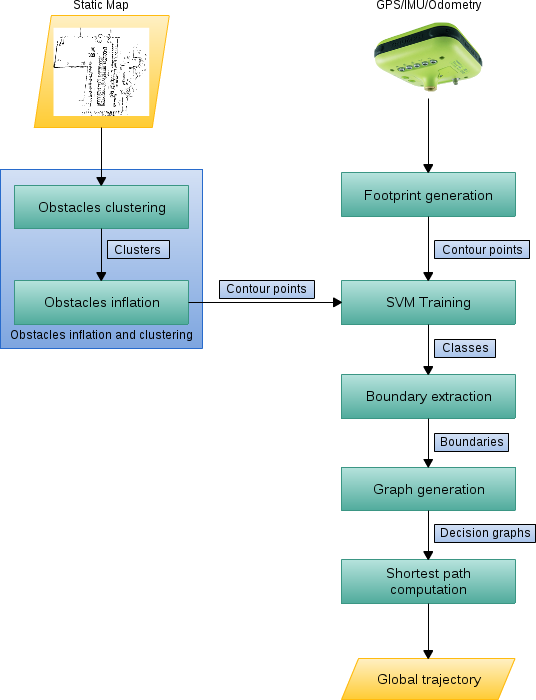
\includegraphics[width=\textwidth, trim=0 0 0 40,clip]{pipeline}
      \caption{ Pipeline followed in the method described in this chapter. }      
      \label{fig:cp06_pipeline}
\end{figure}

In successive iterations, obstacles and the footprint of the vehicle itself will generate a new set of contour points that will be added to the input of the \ac{MSVM}. This way, we just compute the boundaries for the affected obstacles, avoiding to repeat the whole process to the whole map and saving time.

\subsection{First execution}\label{ch:chapter06_01_01}

The generation of the initial graph is composed by the following steps:

\subsubsection{Obstacles Inflation}\label{ch:chapter06_01_01_01}

In our implementation, we have considered the world map as a grid of a given resolution in which obstacles are represented using a value going from 0 to 255, where 0 represents a free area and 255 is an obstacle. Using this map, we calculate the cost for each cell $c(x,y)$ in the map using the following function:

\begin{equation}\label{eq:cp06_cell_cost}
 cost(c) = 253 * \exp( -1 \cdot \beta \cdot (\| nearest(c) - c\| - \rho) )
\end{equation}

, where $\beta$ is a scaling factor that increases/decreases the slope of the cost function, $nearest(c)$ is the position of the nearest cell in the map to the cell $c$ marked as obstacle, and $\rho$ is the circumscribed radius of the robot. The function is scaled to $253$ as 254 and 255 are reserved values. This cost map has been calculated using the \acf{ROS}\footnote{\url{http://www.ros.org}}. Based on the cost map generated, we mark all values over a threshold $\tau$ as obstacle, so the cost map becomes a binary matrix, from which we extract the boundaries using the method in \cite{suzuki1985topological}. In figure \ref{fig:cp06_obst_inflation}, the output after doing this step is shown.

\begin{figure}[h!]
  \centering
  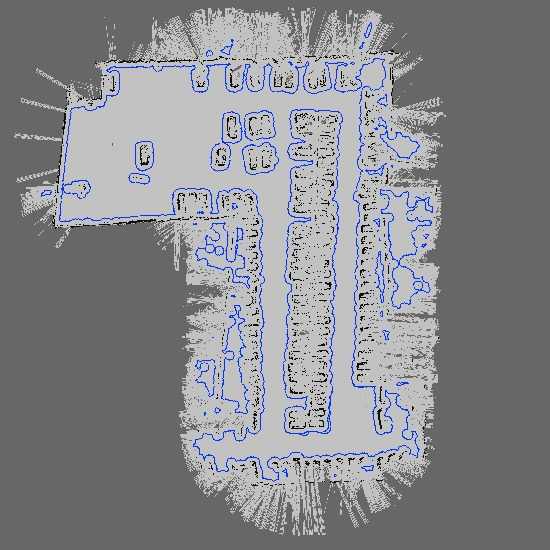
\includegraphics[width=\textwidth, trim=0 0 0 0,clip]{figure1}
  \caption{Obstacles inflation.}
  \label{fig:cp06_obst_inflation}
\end{figure}    

\subsubsection{Obstacles Clustering}\label{ch:chapter06_01_01_02}

The boundaries obtained in the previous step are used as input for the obstacles clustering stage. At this point, we have a cloud of points $\mathcal{P}$ from which we do not know if they belong to the same obstacle or not. This clustering is done using the method described in \cite{rusu2009semantic}. The procedure is the following:

\begin{algorithm}
\caption{Obstacles clustering}
\label{alg:obstacles_clustering}
\begin{algorithmic}
\ForAll{$p_i \in \mathcal{P}$}
  \State add $p_i$ to the queue $\mathcal{Q}$.
  \ForAll{$p_i \in \mathcal{Q}$}
    \State look for the set of neighbors of $p_i$, $\mathcal{P}_i^k$, inside a circle of radius $d_{obst}$.
    \ForAll{$p_i^k \in \mathcal{P}_i^k$}
      \If{\textbf{not} $p_i^k$ is processed}
	\State add $p_i^k$ to $\mathcal{Q}$.
      \EndIf
    \EndFor
    \If {all points in $\mathcal{Q}$ have been processed} 
      \State add $\mathcal{Q}$ to the list of clusters $\mathcal{C}$.
      \State reset $\mathcal{Q}$ to an empty list.
    \EndIf
  \EndFor
\EndFor
\end{algorithmic}
\end{algorithm}

In this algorithm, $d_{obst}$ is the maximal distance between a pair of points to consider them to belong to different obstacles. In our implementation, this step has been developed with the help of the \acf{PCL}\footnote{\url{http://pointclouds.org/}}

\subsubsection{\ac{SVM} Training}\label{ch:chapter06_01_01_03}

Once we have clustered the inflated obstacles into different objects, we want to know which is the best path between them in terms of distance to the obstacles and smoothness. The way in which this is done makes the difference with respect to other \ac{SVM} based path planning algorithms. Unlike the methods seen in section \ref{ch:chapter00_02_06}, our method uses Multiclass \acp{SVM} in order to obtain the best path between the obstacles. In general, in classification, generation of a solution for the multiclass classification in a single step is usually avoided. Instead of this, a combination of several binary \ac{SVM} classifiers is used. The most known methods for doing that, based on the review in \cite{hsu2002comparison, duan2005best}, are:

\begin{itemize}
 \item One-versus all using winner-takes-all.
 \item One-versus-one using max-wins voting.
 \item Directed Acyclic Graph SVM (DAGSVM).
\end{itemize}

In our implementation we used a one-versus-all strategy. That is, for each set of points $C_i$ corresponding to a cluster in the set of clusters $\mathcal{C}$, we create two classes, one formed by the point set $C_i$, and the other composed by the points belonging to the remaining clusters $\{\mathcal{C} - C_i\}$. From these two classes, we train a single \ac{SVM}, which will give us the parameters $\alpha_k$ corresponding to the support vectors $x_k$ and their labels $y_k$, which will be later used by the equation \ref{eq:appendixSVM_soft_discriminative_function}. In our implementation, we used a slightly modified version of the the \acf{GPU}-accelerated LIBSVM libraries, described in \cite{athanasopoulos2011gpu}. The use of these libraries notably improved the time of our implementation.

\subsubsection{Boundary extraction}\label{ch:chapter06_01_01_04}

Once we have obtained the parameters $\alpha_k$, $x_k$ and $y_k$, we need to know where the decision boundary is for each class. That is, based on the equation \ref{eq:appendixSVM_soft_discriminative_function}, we look for the $x$ points that satisfy:

\begin{equation}\label{eq:cp06_decision_boundary}
 y = \sum_{k \in S} \alpha_k y_k K(x_k, x) + b = 0
\end{equation}

These points will allow us obtaining a non-linear decision curve. In figure \ref{fig:cp06_decision_boundary_3d}, we have represented, for each cell $(x,y)$ in a map, the values obtained from equation \ref{eq:cp06_decision_boundary} as their $Z$ coordinate, using the parameters obtained after training a given class. The plane represented in black is $Z=0$, so all cells in which this plane intersects with the named function will belong to a path.
In fact, as solving the equation \ref{eq:cp06_decision_boundary} can be too computationally expensive, the way in which we have implemented this is as follows: First, we sample the map into a grid of a given resolution. For each cell in the map, we obtain the value given by equation \ref{eq:cp06_decision_boundary}. If positive, we assign $1$ to this cell. Else, we assign $0$. This process is executed over the \ac{GPU} using a \ac{CUDA} function developed for this purpose, so it is fully parallelized, taking a very small amount of time to be executed.

\begin{figure}[h!]
  \centering
  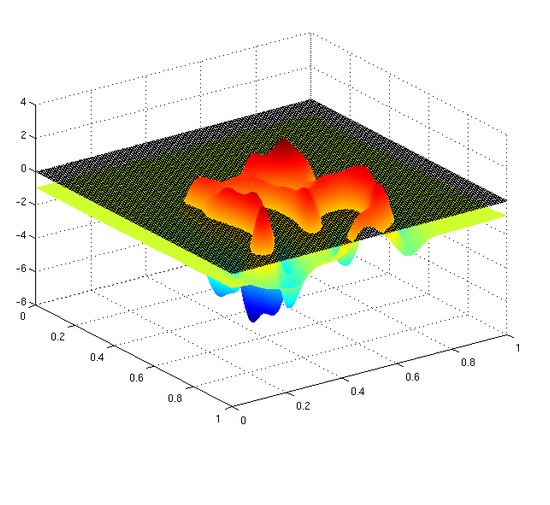
\includegraphics[width=\textwidth, trim=0 0 0 0,clip]{figure2}
  \caption{Output of \ref{eq:cp06_soft_discriminative_function} for a given class.}
  \label{fig:cp06_decision_boundary_3d}
\end{figure}

Once we have create our new map, we extract our boundaries using again the method in \cite{suzuki1985topological}. We store the points in a point set $\mathcal{B}$, which will be shared by all classes. At this point we do not store neighborhood information, but we add to each point $p_i$ a label $l_i$ in order to know the class from which they were generated initially. This information will be used in the graph generation stage.

\subsubsection{Graph generation}\label{ch:chapter06_01_01_05}

The graph generation stage takes as input the points in $\mathcal{B}$ and tries to generate a connectivity graph that will be used later to obtain the shortest paths between pairs of points in the map. At a first glance, this stage is as simple as connecting all the points generated by the same class together, and joining those subgraphs by the points in which the decision boundaries cross each other. Unfortunately, it is not as simple as seems, because there are situations where there is a big area free of obstacles, which avoids the connections between to classes, making it impossible to travel from the path belonging to one class to the other using this first approach. This effect can be observed for some of the obstacles represented in figure \ref{fig:cp06_nng}.
To solve this problem, in our method we propose a combination of a \acf{RNG} based on the Delaunay triangulation (\cite{lingas1994linear}), and a \acf{NNG} (\cite{eppstein1997nearest}).

\paragraph{\acf{NNG}}\label{ch:chapter06_01_01_05_01}

In order to obtain the \ac{NNG}, we calculate a $kd-tree$ for the points in $\mathcal{B}$. For each point in $\mathcal{B}$, we look for the neighbors inside a given radius circle. Then an edge $e(u,v)$ is added to the graph for each point in the circle, where $u$ is the current point, and $v$ each one of the neighbors of $u$. By doing this, we allow the robot to go from the path obtained from a class to another in case points are close enough and there are no obstacles in the neighborhood. In figure \ref{fig:cp06_nng}, we can see the graph as it would look like at this point of the execution. As can be seen, there are some boundaries that are not connected, despite that there is a free area between them. This problem is solved with the \acf{RNG}.

\begin{figure}[h!]
  \centering
  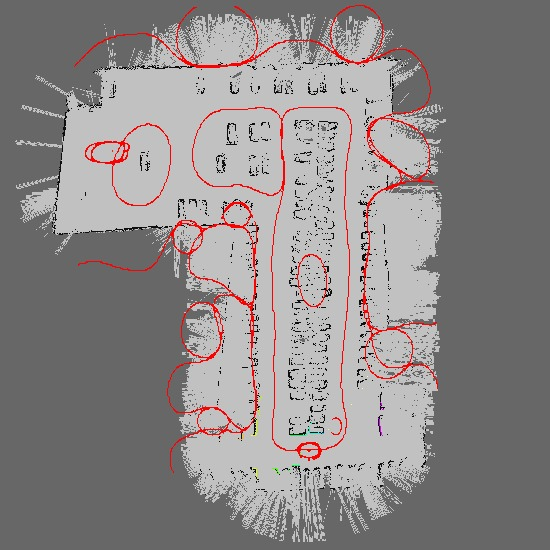
\includegraphics[width=\textwidth, trim=0 0 0 0,clip]{figure3}
  \caption{\acf{NNG}.}
  \label{fig:cp06_nng}
\end{figure}

\paragraph{\acf{RNG}}\label{ch:chapter06_01_01_05_02}

For the generation of the \ac{RNG}, we use the set of labels $l_i \in \mathcal{L}$ described in section \ref{ch:chapter06_01_01_04}. First, we obtain the Delaunay Triangulation \cite{su1997comparison} using the points in $\mathcal{B}$ as input. In our implementation, we used the method in \cite{rong2008computing} for that. Then, we iterate through the edges $e(u,v)$ of the triangles. For each one of these edges, we look for the nearest point belonging to an obstacle. If the point is far enough and $l_u \neq l_v$, we add the edge to our graph. In our implementation, we have developed some code that processes all edges at the same time over the \acf{GPU}, allowing to save a lot of time in a process that would be too expensive in a sequential implementation. Edges obtained by the \ac{NNG} are tested, too. The obtained graph is depicted in figure \ref{fig:cp06_rng}.

\begin{figure}[h!]
  \centering
  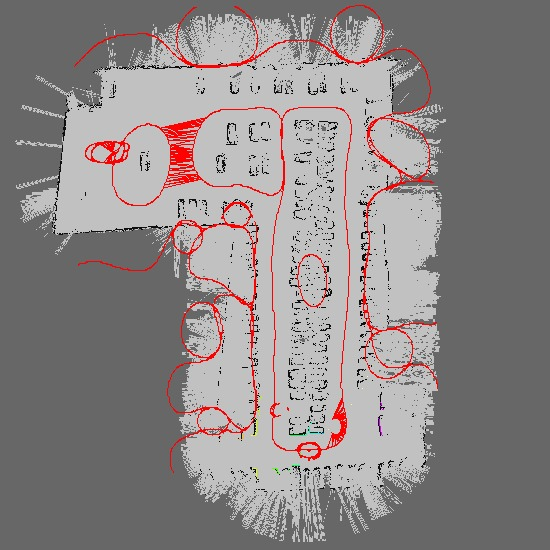
\includegraphics[width=\textwidth, trim=0 0 0 0,clip]{figure4}
  \caption{\acf{RNG}.}
  \label{fig:cp06_rng}
\end{figure}%

At this point, we have a graph that allows us going from any point in the map to another ensuring a safe and smooth path. However, in successive iterations, there could be obstacles that were not there when the initial map was created, so the graph must be updated in the following executions. The process that solves this situation is explained in the following section.

\subsection{Successive executions}\label{ch:chapter06_01_02}

The steps in the successive executions are quite similar to those in the initial execution. However, for optimization purposes, we do not need to recalculate the whole map in each execution, but extend the map we had from the previous one. The steps needed are the following.

\subsubsection{Obstacles Inflation and clustering}\label{ch:chapter06_01_02_01}

The step of obstacles inflation is exactly the same as that described in section \ref{ch:chapter06_01_01_01}. The only difference is that points from the inflation boundary are compared to those in the original map. To do that, we calculate a $kd-tree$ from the set of points obtained in the first execution, $\mathcal{O}_{old}$. Then, for each point $o_i$ in the new set, $\mathcal{O}_{new}$, we look for the nearest point in $\mathcal{O}_{new}$. If the nearest point of $o_i$ is nearer than a given threshold, it is removed from $\mathcal{O}_{new}$. Then, the clustering step is performed similarly as happened in the first execution, but with the filtered set $\mathcal{O}_{new}$.

\subsubsection{Footprint generation}\label{ch:chapter06_01_02_02}

We want to get the path starting from an initial point towards to a goal. To do this, we need to add a pair of fake obstacles that helps to generate the trajectory the robot will follow from its current position towards the nearest point in the graph, and from the graph to the goal. Also, these fake obstacles will prevent the robot to start traveling in an impossible angle given its current orientation. The same applies for the desired goal position and orientation. Before starting all the process, we check that we are not currently colliding with an obstacle. In this case, the process is aborted and recovery behaviors should be triggered. If everything is right, we generate a set of points ($\mathcal{F}_L$) that go from the position $A(-\rho, +\rho)$ to the position $B(\rho, \rho)$, and another one ($\mathcal{F}_R$) coming from $C(-\rho, -\rho)$ to $D(\rho, -\rho)$, being $\rho$ the circumscribed radius of the robot defined in section \ref{ch:chapter06_01_01_01}. 

\begin{figure}[h!]
  \centering
  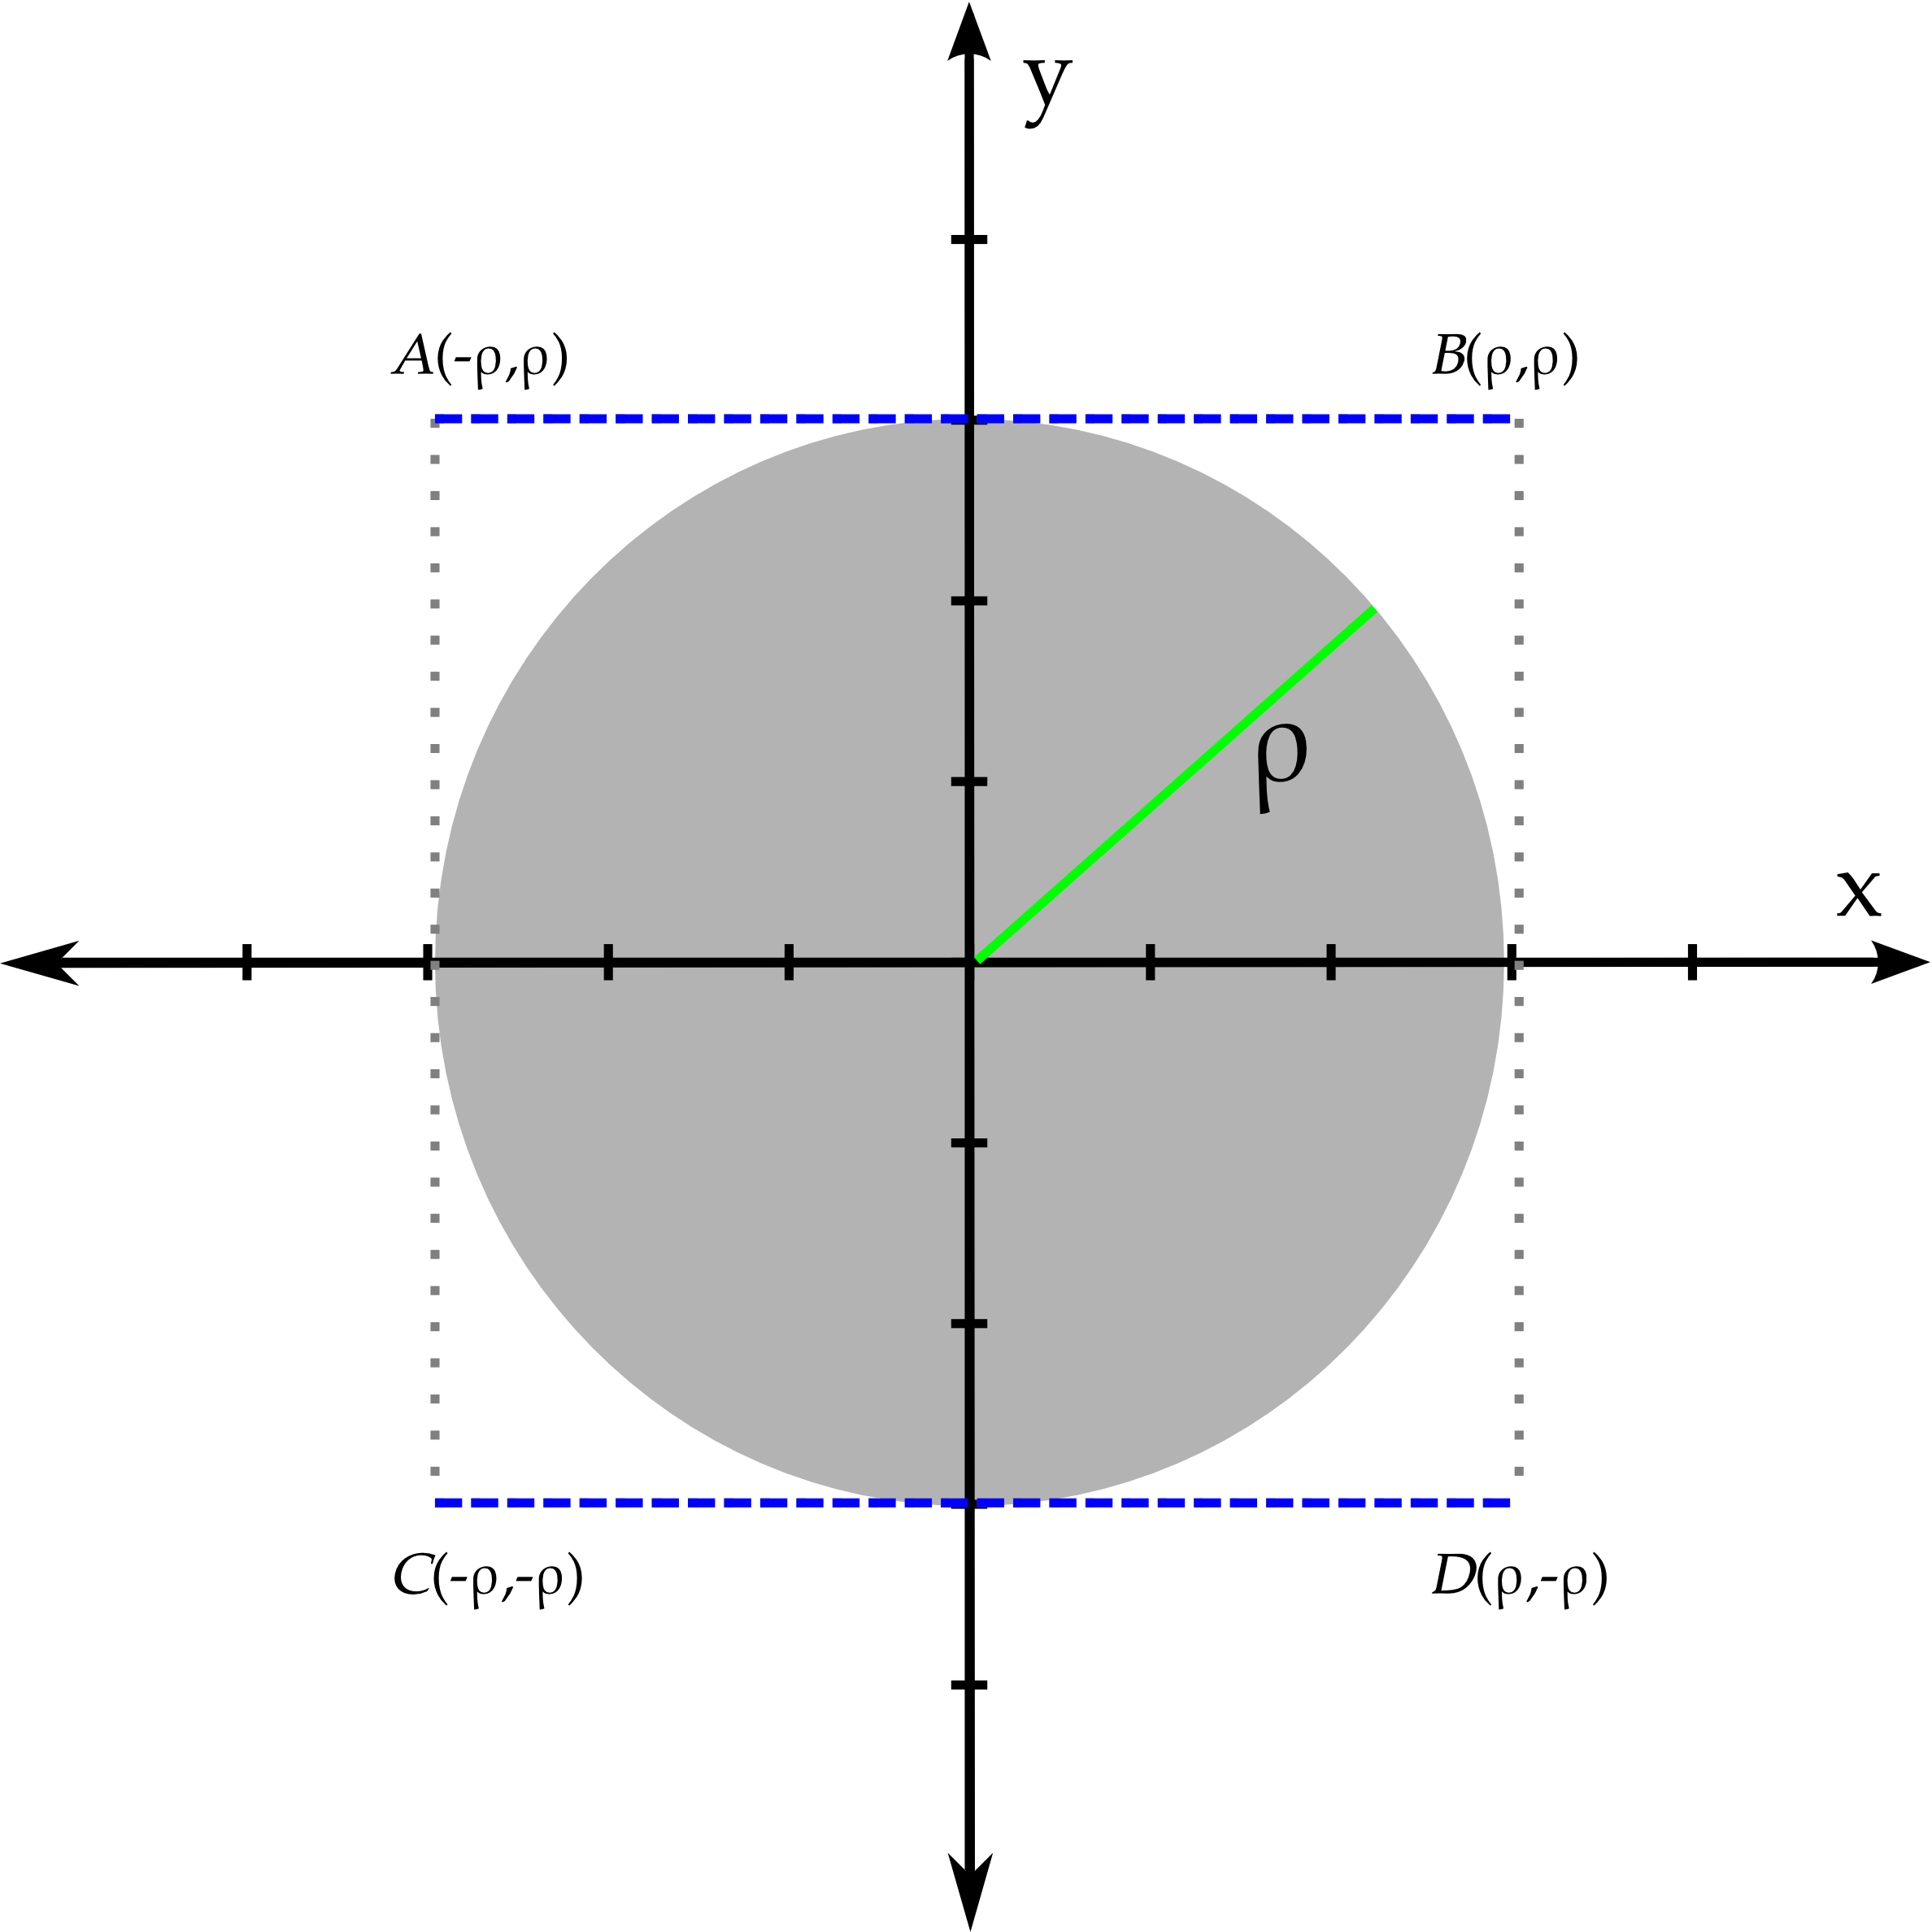
\includegraphics[width=\textwidth, trim=0 0 0 0,clip]{figure5}
  \caption{Footprint generation.}
  \label{fig:cp06_footprint_generation}
\end{figure}%

In figure \ref{fig:cp06_footprint_generation}, this process is represented, as well as points $A$, $B$, $C$ and $D$. Each point set represents a class for the following steps in the method. Coordinates of the obtained point sets $\mathcal{F}_L$ and $\mathcal{F}_R$ are relative to the robot position, so we must transform them to map coordinates using the transformation matrix

\begin{equation}\label{eq:cp06_Rt_footprint}
 Rt = \left ( \begin{array}{ ccc }
  \cos(\theta_s) & -\sin(\theta_s) & s_x \\
  \cos(\theta_s) & -\sin(\theta_s) & s_y \\
  0 & 0 & 1
 \end{array} \right )
\end{equation}

, where $s(x,y)$ is the starting point (the current point of the robot), and $\theta_s$ its orientation. Once we have $Rt$, each point $f_{L,i} \in \mathcal{F}_L$ is transformed so its new position $f'_{L,i}$ becomes ${f'}_{L,i}^T = Rt \cdot f_{L,i}^T$. Same applies to the points in $\mathcal{F}_R$.

The same process is performed for the goal point $g(x,y)$ and its orientation $\theta_g$. As it can be noticed, we have limited the orientation of the vehicle in the start and goal points, but not the direction. This limitation will be fulfilled in the process described in section \ref{ch:chapter06_01_02_04_01}. This could have been done also by closing the obstacle by joining the points $A$ and $C$ with a new set of points, but there is a risk of having imprecise decision boundaries, which could make the algorithm not to find a feasible path.

\subsubsection{\ac{SVM} training, boundary extraction and graph generation}\label{ch:chapter06_01_02_03}

Once we have the classes corresponding to the new points obtained by the sensors of the robot, together with the four classes corresponding to the footprints, the stages of \ac{SVM} training, boundary extraction and graph generation are exactly the same described in sections \ref{ch:chapter06_01_01_03}, \ref{ch:chapter06_01_01_04} and \ref{ch:chapter06_01_01_05}. As it would be expected, we remove the paths that were in the original graph but that are not longer traversable due to the presence of obstacles.

\subsubsection{Shortest path calculation}\label{ch:chapter06_01_02_04}

At this point, we have a graph with all the feasible paths in the map totally updated, including the new obstacles that could be in the way. With this graph, it is possible to find a safe and smooth path between the given starting and goal positions and their orientations.

\paragraph{Looking for the starting and goal points into the graph}\label{ch:chapter06_01_02_04_01}

As said in section \ref{ch:chapter06_01_02_02}, we have limited the robot to start with a given orientation, but at this point we are not taking into account its direction. To solve this, given the current position of the robot and the goal, $s(x,y)$ and $g(x,y)$, and their orientations, $\theta_s$ and $\theta_g$, we obtain the points

\begin{equation}\label{eq:cp06_start_goal_points}
\begin {array}{l}
 s_1 = (s_x + \rho * \cos(\theta_s), s_y + \rho * \sin(\theta_s)) \\
 g_1 = (g_x - \rho * \cos(\theta_g), g_y - \rho * \sin(\theta_g))
\end{array}
\end{equation}

Then, we use the points $s_1$ and $g_1$ to look for the nearest point in the graph, using the kd-tree previously created in the previous sections. These nearest points, $s_2$ and $g_2$, will be the points used by Dijkstra to find a path. This operation is better described in figure \ref{fig:cp06_findstartgoal}. In this figure, using the current position of the robot (starting point $s$), represented in red, and its orientation, we obtain the point $s_1$ (the point in magenta) based on the equation \ref{eq:cp06_start_goal_points}. In the graph, the nearest point to $s_1$ (pink), $s_2$ (dark blue), is the initial point that will be used as input for the Dijkstra algorithm.

\begin{figure}[h!]
  \centering
  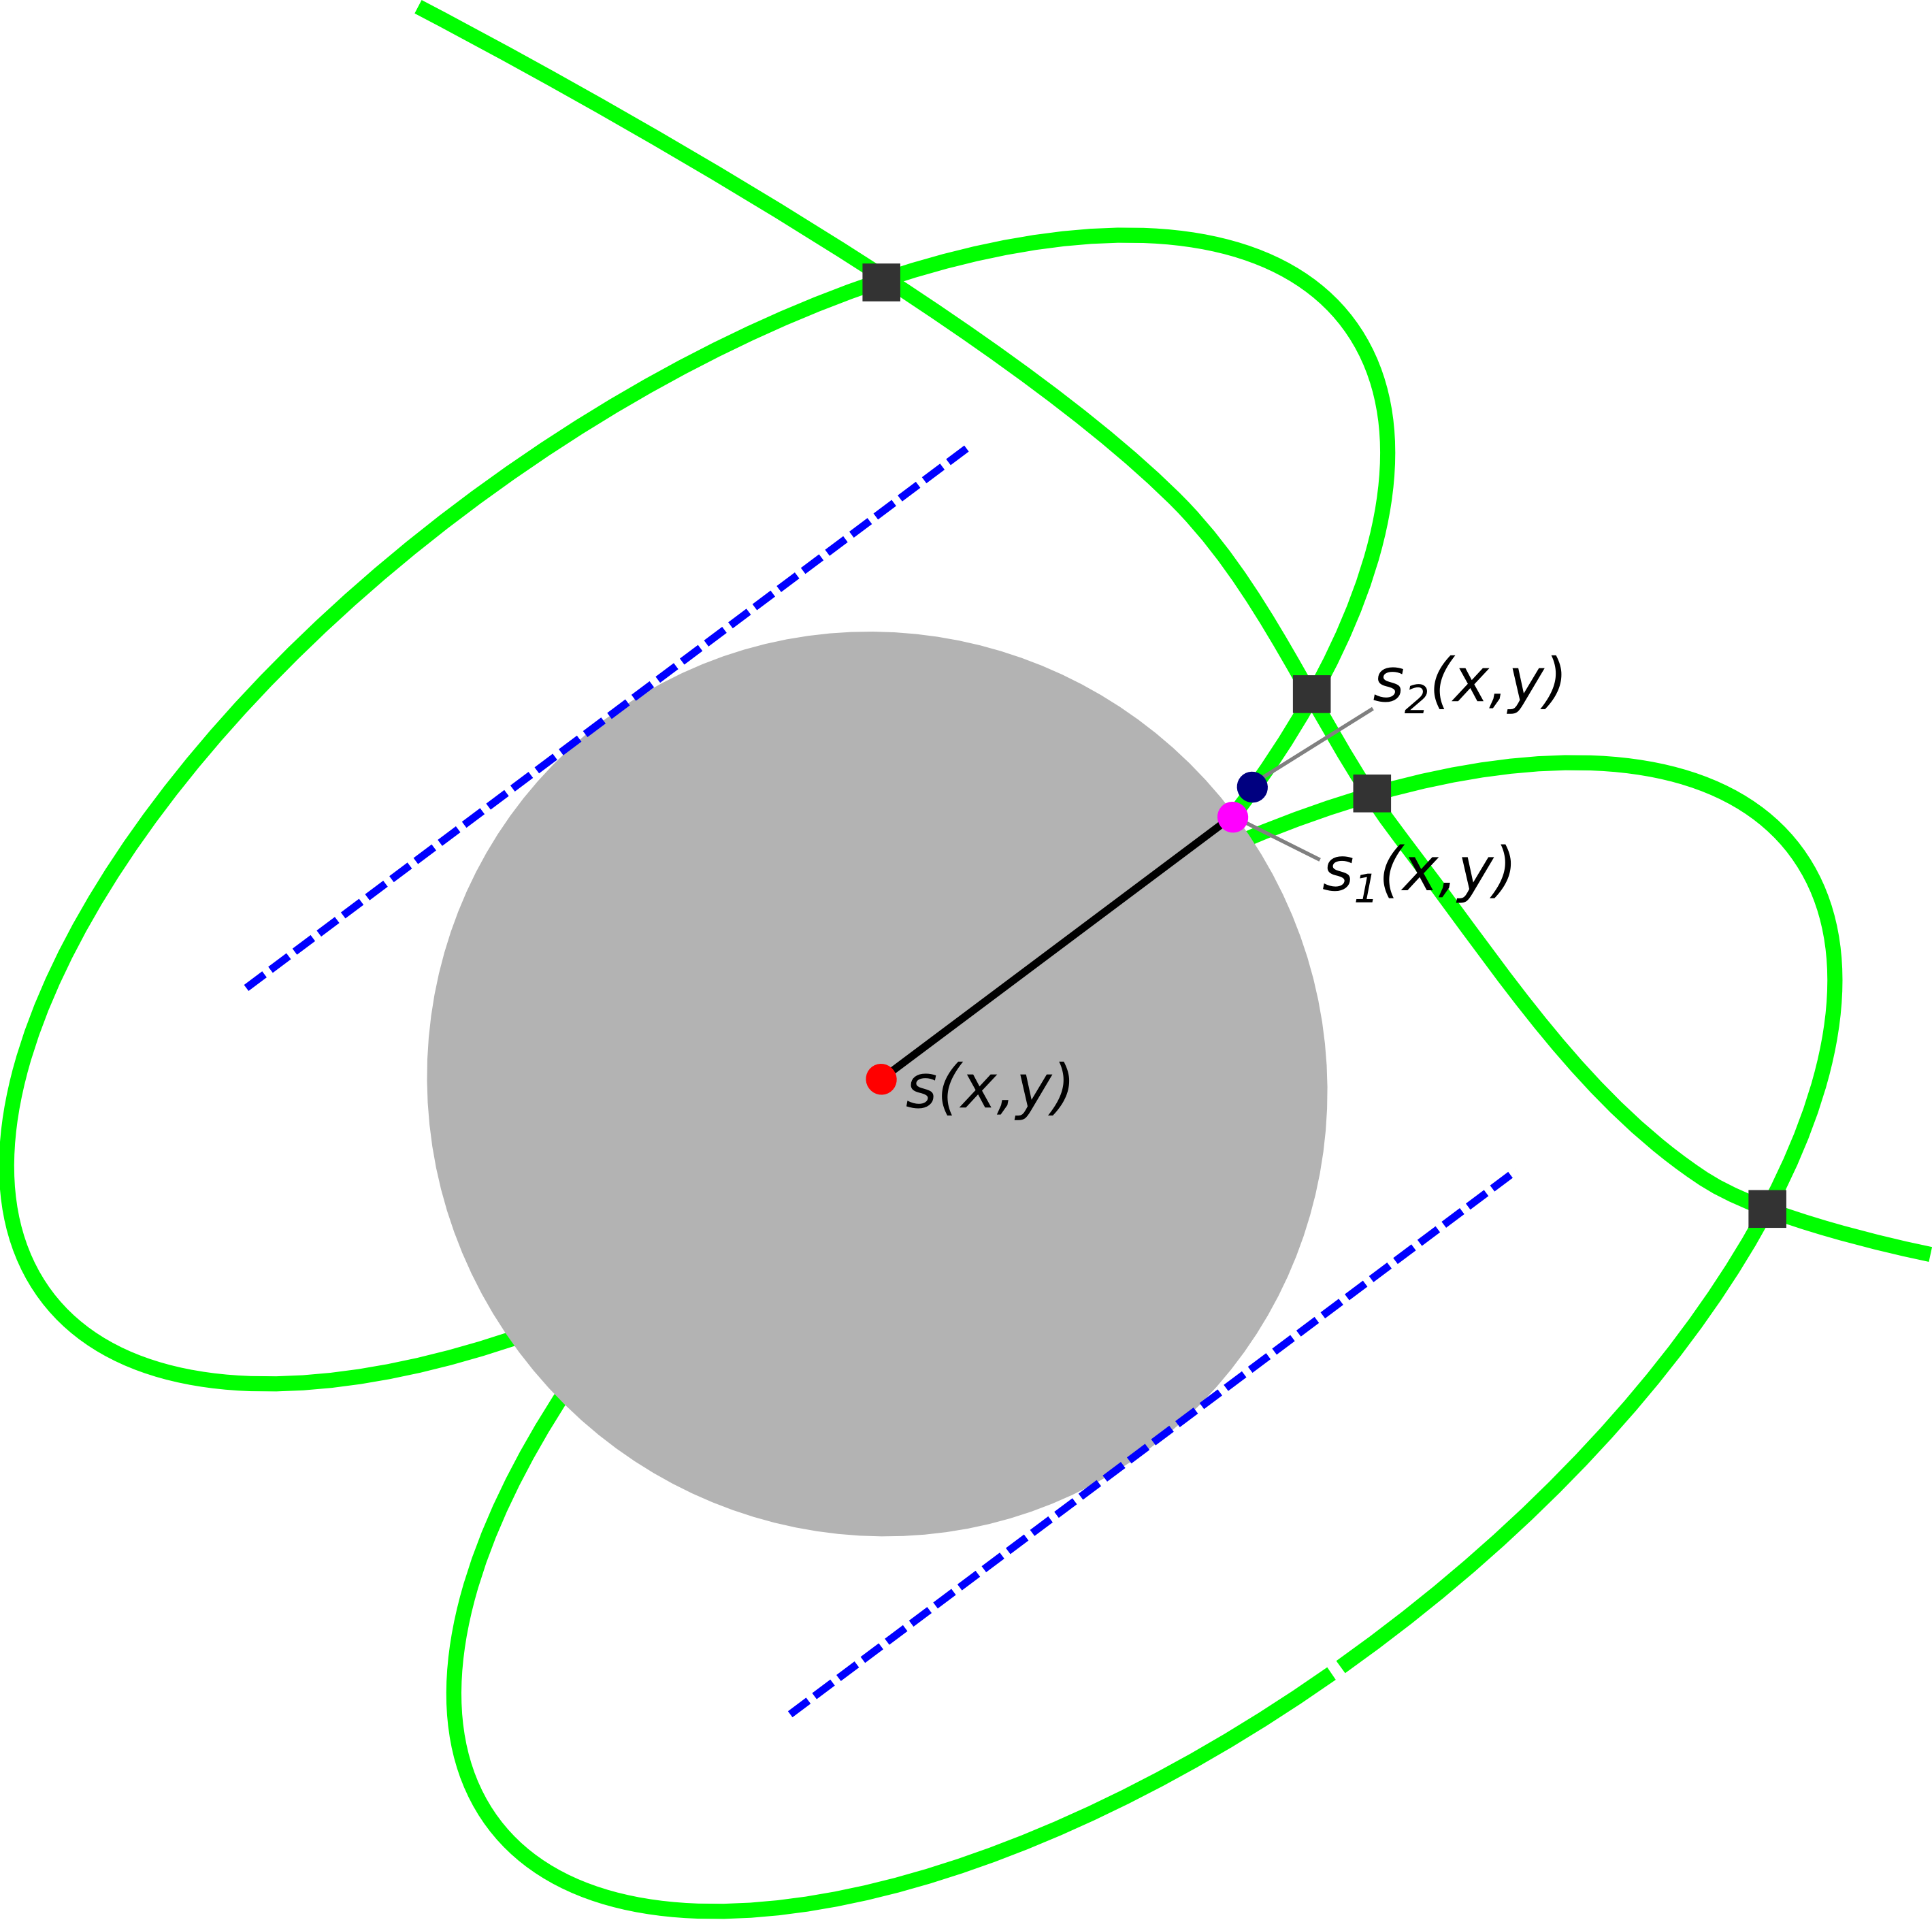
\includegraphics[width=\textwidth, trim=0 0 0 0,clip]{figure6}
  \caption{Starting and goal point selection process.}
  \label{fig:cp06_findstartgoal}
\end{figure}

\paragraph{Looking for the shortest path}\label{ch:chapter06_01_02_04_02}

Before applying Dijkstra to find the shortest path, we need to know if the goal is reachable. To do that, we check the connectivity of the graph. If $s_2$ and $g_2$ are in the same connected component, the goal is reachable. This checking is needed because, due to some of the decisions made for the previous stages and as shown in figure \ref{fig:cp06_rng}, there will be a graph in every place in which there is a hole between the limits obtained in the obstacles inflation step. This is because we do not consider the real obstacles like solid parts, but just the boundary limit after the inflation. However, it is faster making a connectivity checking than testing whether a graph is in a traversable area or not. We suppose that the robot will always start in a valid area.
Once we have done this verification, Dijkstra is applied over the graph and the path is obtained. Points $s$ and $g$ are added to the beginning and the end of the path. In our implementation, all graph-related methods have been implemented using LEMON libraries\footnote{\url{http://lemon.cs.elte.hu}}. The whole implementation of the algorithm has been tested on a PC i7-3630QM with 8GB RAM and a NVIDIA GT 640M, being able to work in a real time navigation application for an autonomous robot, giving an average time of 1.6\ seconds for each iteration.

Some improvements could be incorporated to the current method, like using the extended \ac{SVM} version described in \cite{qingyang2012local}, which would allow satisfying additional restrictions, such as the robot position or heading. Also, the path generated by our method could be smoothed again using a second \ac{SVM} step, as done for the path generated by the Voronoi diagrams in \cite{yang2012safe}.

In figure \ref{fig:cp06_final_path}, the final path obtained by the algorithm is shown. In the next section, some results are shown, demonstrating the good behavior of the method, comparing it with some of the best algorithms that use \ac{SVM} for path planning.

\begin{figure}[h!]
  \centering
  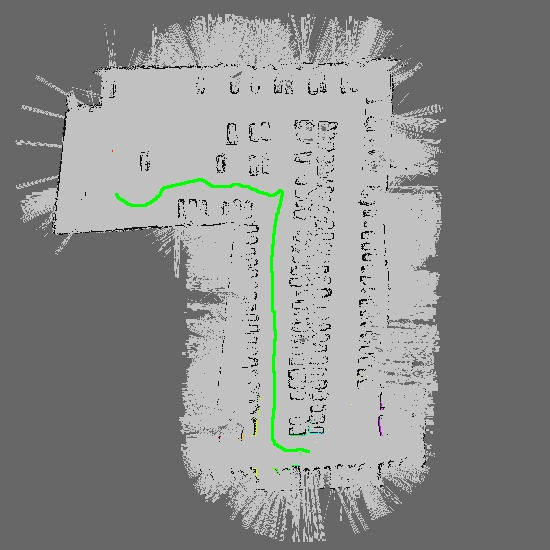
\includegraphics[width=0.4\textwidth, trim=0 0 0 0,clip]{figure7}
  \caption{Final path.}
  \label{fig:cp06_final_path}
\end{figure}


\section{Results}\label{ch:chapter06_02}

This section shows the results obtained from two different experiments performed in order to validate the good response of the method. In section \ref{ch:chapter06_02_01}, we show the results obtained when trying to get the best parameters for our method. In section \ref{ch:chapter06_02_02}, we compare our method with other related methods found in the literature.

\subsection{Parameterization}\label{ch:chapter06_02_01}

The first set of experiments tries to to find the best parameters for our method. We have stored several paths obtained with a given parameterization in a real scenario. In particular, we have tested the quality of the generated paths when parameters $C$ of the equation \ref{eq:appendixSVM_soft_objective_function} and $\gamma$ of the \ac{RBF} kernel are modified. For each set of paths, we have performed the following measures:

\begin{figure*}[h!]
  \centering
  \begin{subfigure}[b]{\textwidth}
	  \centering
	  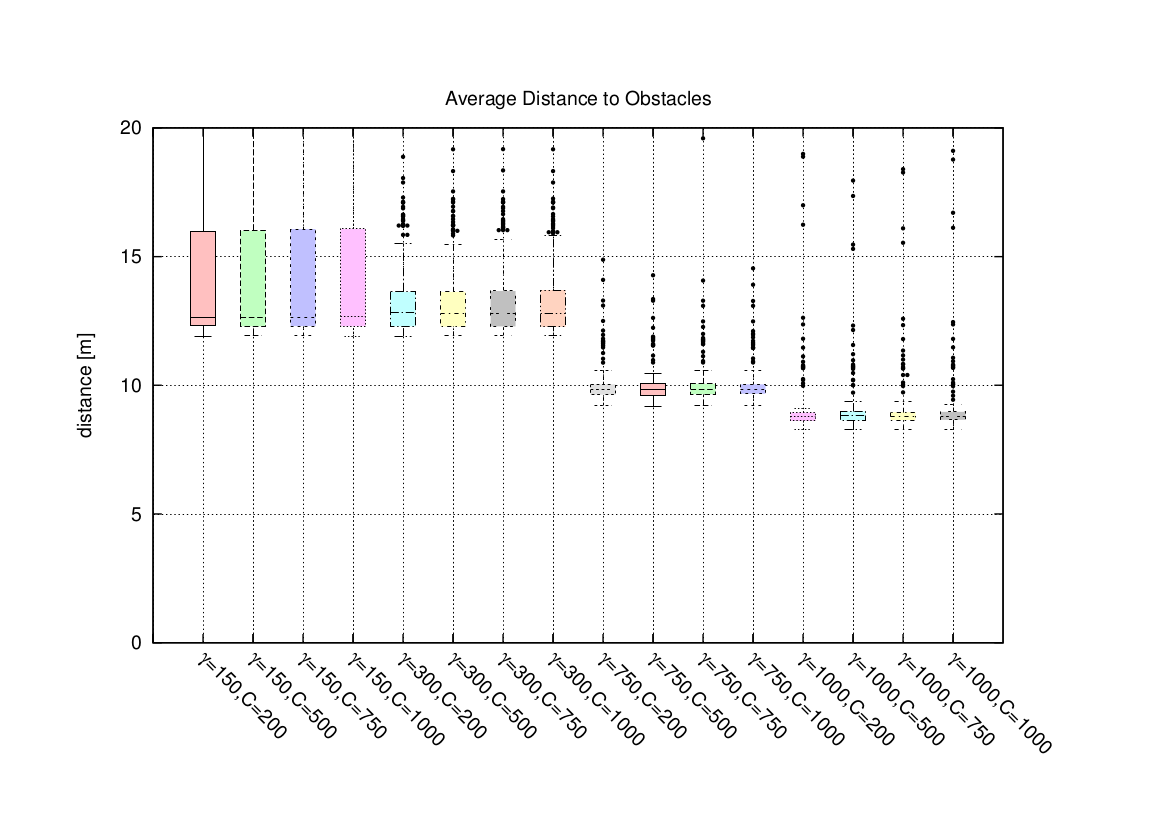
\includegraphics[width=\textwidth, trim=55 50 85 60,clip]{figure8}
	  \caption{Average distance to obstacles.}
	  \label{fig:cp06_avg_dist_msvmpp}
  \end{subfigure}  

  \begin{subfigure}[b]{\textwidth}
	  \centering
%                 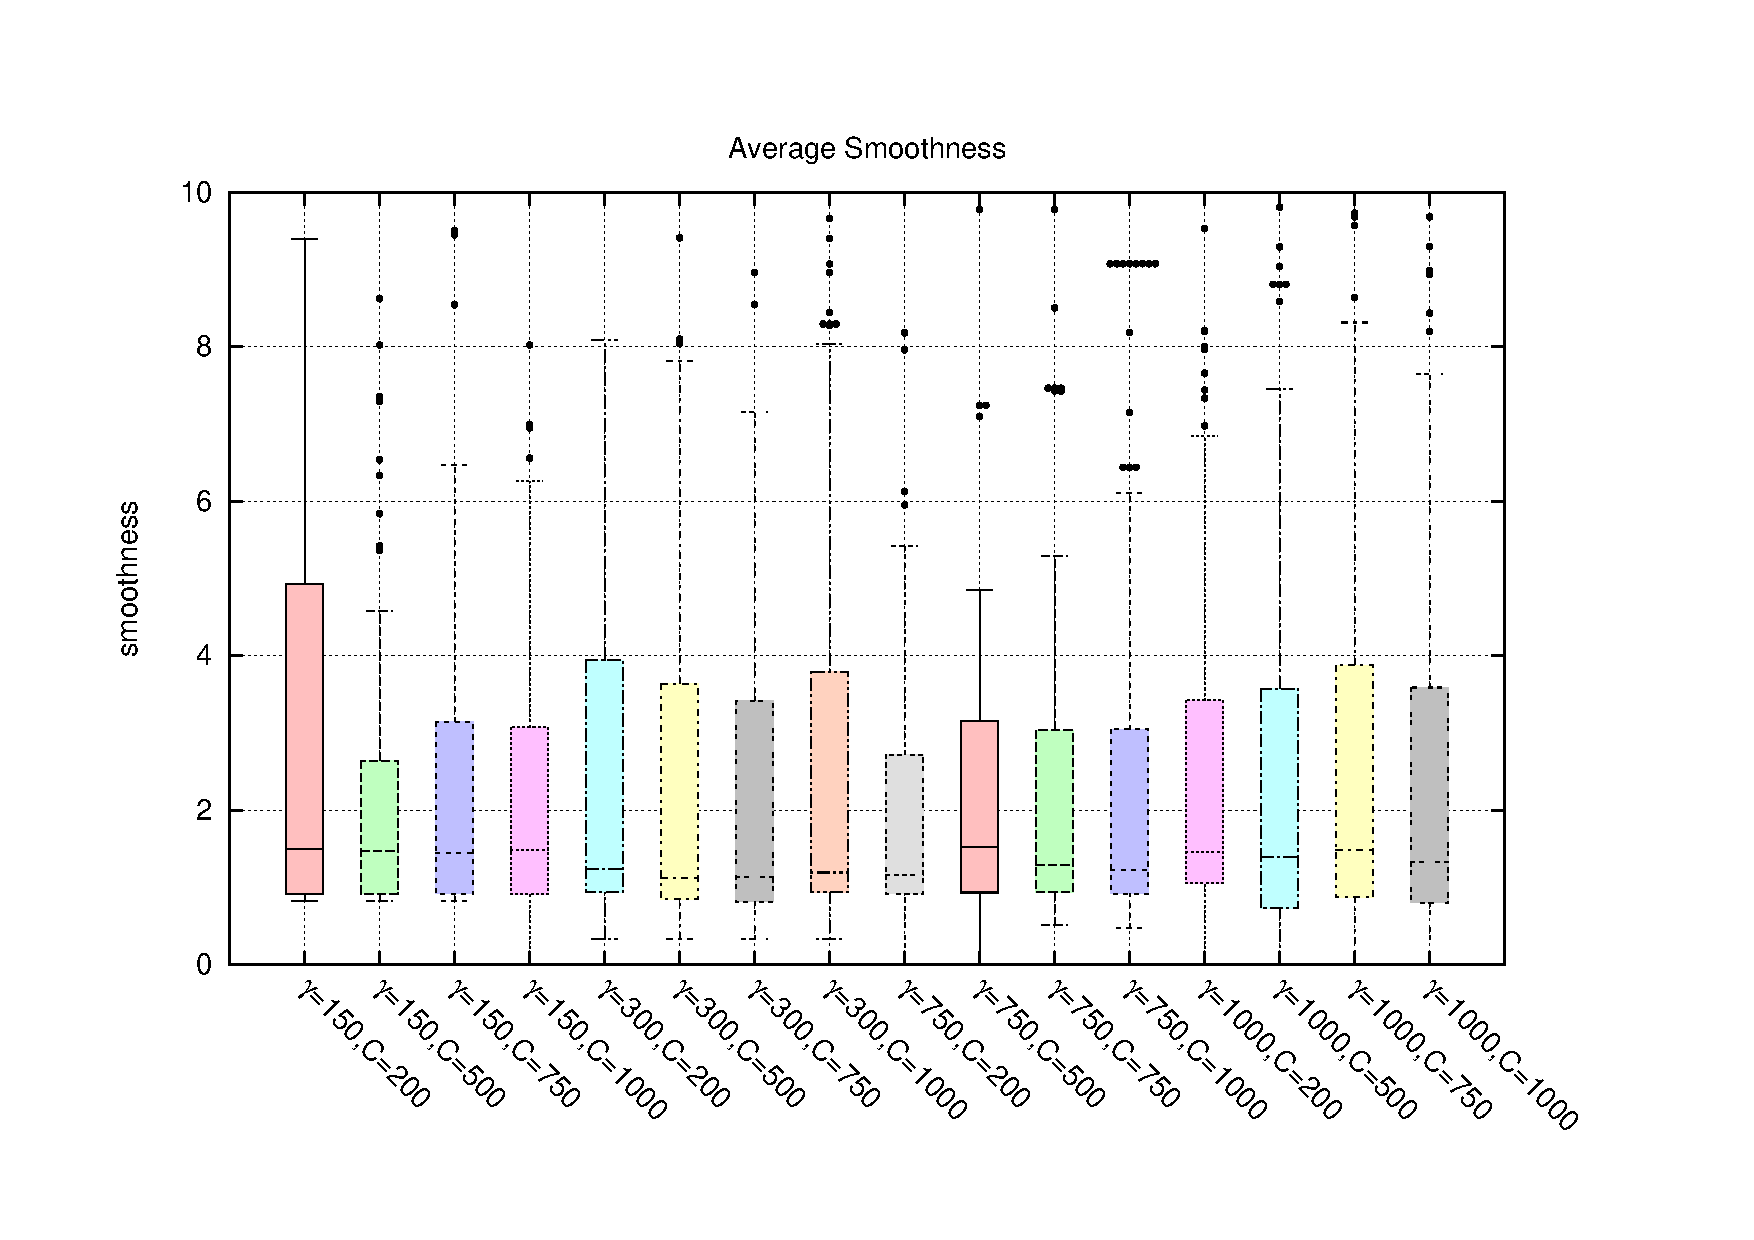
\includegraphics[width=\textwidth, trim=55 50 85 60,clip]{figures/avgSmooth_MSVMPP}
	  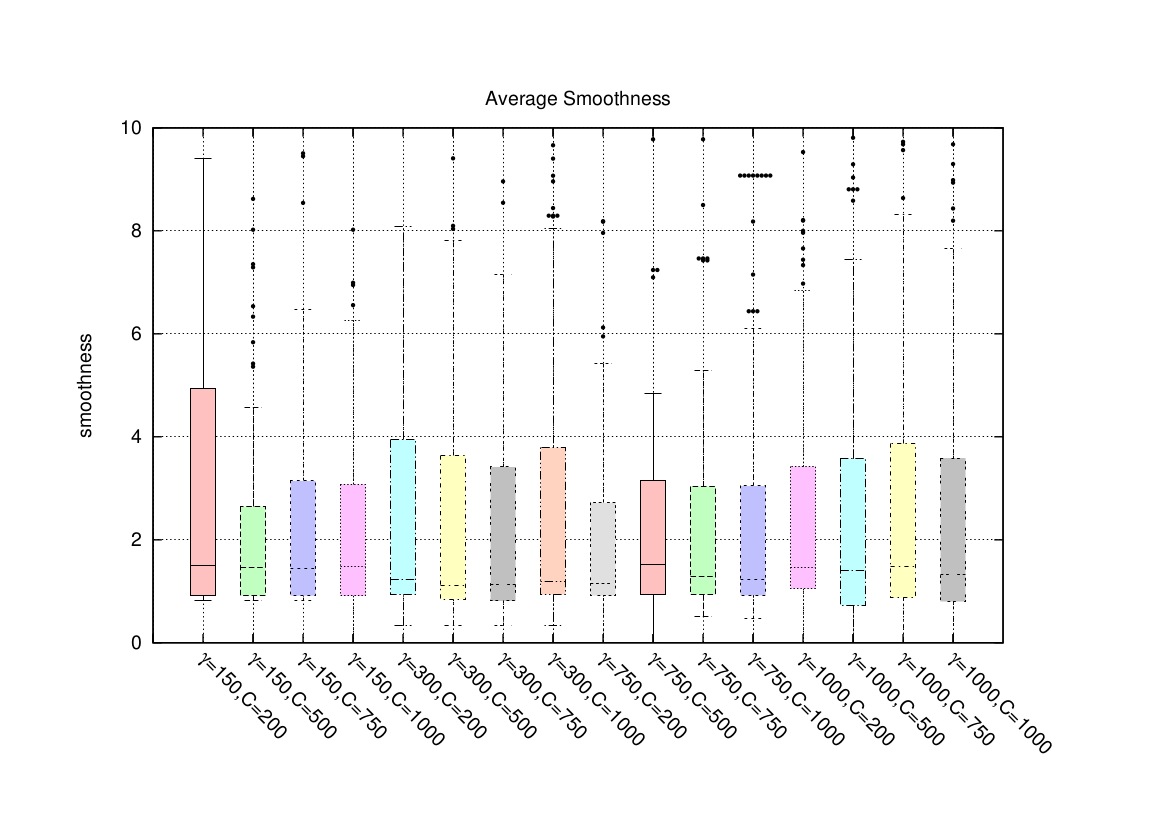
\includegraphics[width=\textwidth, trim=55 50 85 60,clip]{figure9}
	  \caption{Smoothness.}
	  \label{fig:cp06_smoothness_msvmpp}
  \end{subfigure}        
  \phantomcaption % new inserted command
\end{figure*}

\begin{figure*}
  \ContinuedFloat
  \begin{subfigure}[b]{\textwidth}
	  \centering
%                 \includegraphics[width=\textwidth, trim=55 40 85 60,clip]{figures/Length_MSVMPP}
	  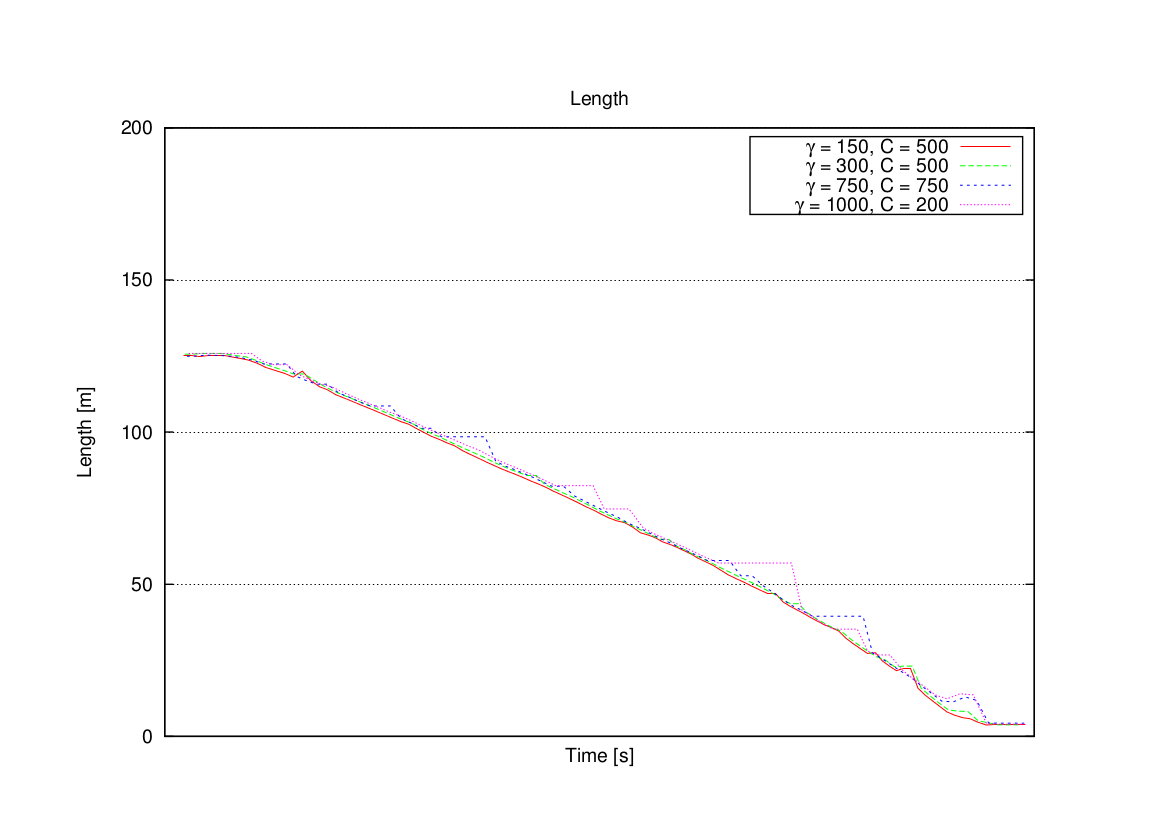
\includegraphics[width=\textwidth, trim=55 50 85 60,clip]{figure10}
	  \caption{Length.}
	  \label{fig:cp06_length_msvmpp}
  \end{subfigure}
  
  \caption{Results obtained for the parameterization of the method.}\label{fig:cp06_results_parameterization}
\end{figure*}

\subsubsection{Average distance to obstacles}\label{ch:chapter06_02_01_01}
Given a set of trajectories $\mathcal{T}$, for each trajectory $t_i$, we obtain the average distance to the nearest obstacle, using the equation

\begin{equation}\label{eq:cp06_avg_dist}
  \bar{d} = {1 \over N_{t_i}} \sum_{j=1}^{N_{t_i}} \| p_j - nearest\_obst(p_j) \|
\end{equation}

, where $N_{t_i}$ is the number of points in the trajectory $t_i$, $nearest\_obst(p_j)$ is the nearest point to the point $p_j$ belonging to and obstacle, and $\| x - y \|$ is the euclidean distance between $x$ and $y$.

In figure \ref{fig:cp06_avg_dist_msvmpp}, we show a chart with a selection of the best results obtained. We have tested values going from 10 to 10000, but for the sake of clarity, just best results are shown. As can be observed, results are more dependent to the $\gamma$ value than to the $C$ parameter. This is due to the fact that the \ac{RBF} kernel is responsible of giving non-linearity to the \ac{SVM}. Best results were obtained with $\gamma = 150$. Best $C$ value is not clear and must be decided with the following tests.

\subsubsection{Smoothness}\label{ch:chapter06_02_01_02}

The other measure we have obtained is the smoothness of the path. The way in which we do that is by averaging the second derivative of each trajectory $t_i$, so the nearest a test is to $0$, the better. In our case,

\begin{equation}\label{eq:cp06_avg_smooth}
  \bar{s} = {1 \over N_{t_i}} \sum_{j=2}^{N_{t_i} - 1} \left[ {{p_j(y) - p_{j-1}(y)} \over {p_j(x) - p_{j-1}(x)}} - {{p_{j + 1}(y) - p_j(y)} \over {p_{j + 1}(x) - p_j(x)}} \right]^2
\end{equation}

, where $p_j(x)$ is the $x$ component of the point $p_j$ in the trajectory $t_i$, and $p_j(y)$ the corresponding $y$ component. In figure \ref{fig:cp06_smoothness_msvmpp}, we can see a chart where a selection of the best $\gamma$ and $C$ values is shown. Best results were obtained for $\gamma=750$, but also $\gamma=150$ has a good behavior, so we remain using this value as it shows a more stable response in all tests. About $C$, the best value is found when $C=500$. So, we have a best parameterization candidate: $C=500$, $\gamma=150$.

\subsubsection{Length}\label{ch:chapter06_02_01_03}

The length of each path has also been tested, where

\begin{equation}\label{eq:cp06_length}
  l = \sum_{j=2}^{N_{t_i}} \| p_j - p_{j - 1}\|
\end{equation}

In our tests, we have launched a execution in which a robot ask for a goal. The robot recalculates the path repeatedly while approaching to this goal. Then, length should decrease monotonically along the time. This behavior is shown in the chart of figure \ref{fig:cp06_length_msvmpp}, where the length output selection of the parameters analyzed in the previous tests is depicted. Best parameters should have a constant approach to zero, while worst show a zigzagging approach. Again, the combination $C=500$, $\gamma=150$ seems to be a good choice.

\subsection{Comparison with other related methods}\label{ch:chapter06_02_02}

In order to demonstrate the good behavior of our method, we have compared it with other related methods that use \ac{SVM} for path planning. In particular, we have implemented the method in \cite{miura2006support}, which will be referenced from now as \textit{Single \ac{SVM}}. As said in section \ref{ch:chapter00_02_06}, this method uses a single \ac{SVM} which is calculated by testing several labeling patterns of the obstacles, incorporating them into one or another class randomly; also, we have implemented the method in \cite{yang2012safe}, which will be referred as \textit{Voronoi+\ac{SVM}}, that pre-generates a path using a Voronoi diagram, which is smoothed using a \ac{SVM}. We have not considered other methods like \cite{sarkar2008mobile} or \cite{qingyang2012local} as they do not analyze the whole map of the environment of the robot but a local window inside it, so results are not comparable. As an example of a classic method, we have included the path planning based Voronoi algorithm, too.
For both \textit{Single \ac{SVM}} and \textit{Voronoi+\ac{SVM}} algorithms, we have performed similar tests to those described in section \ref{ch:chapter06_02_01}. After that, we chose the parameters $C=300$ and $\gamma=200$ for the former, and $C=500$ and $\gamma=750$ for the later.

\begin{figure*}[h!]
  \centering
  \begin{subfigure}[b]{\textwidth}
	  \centering
	  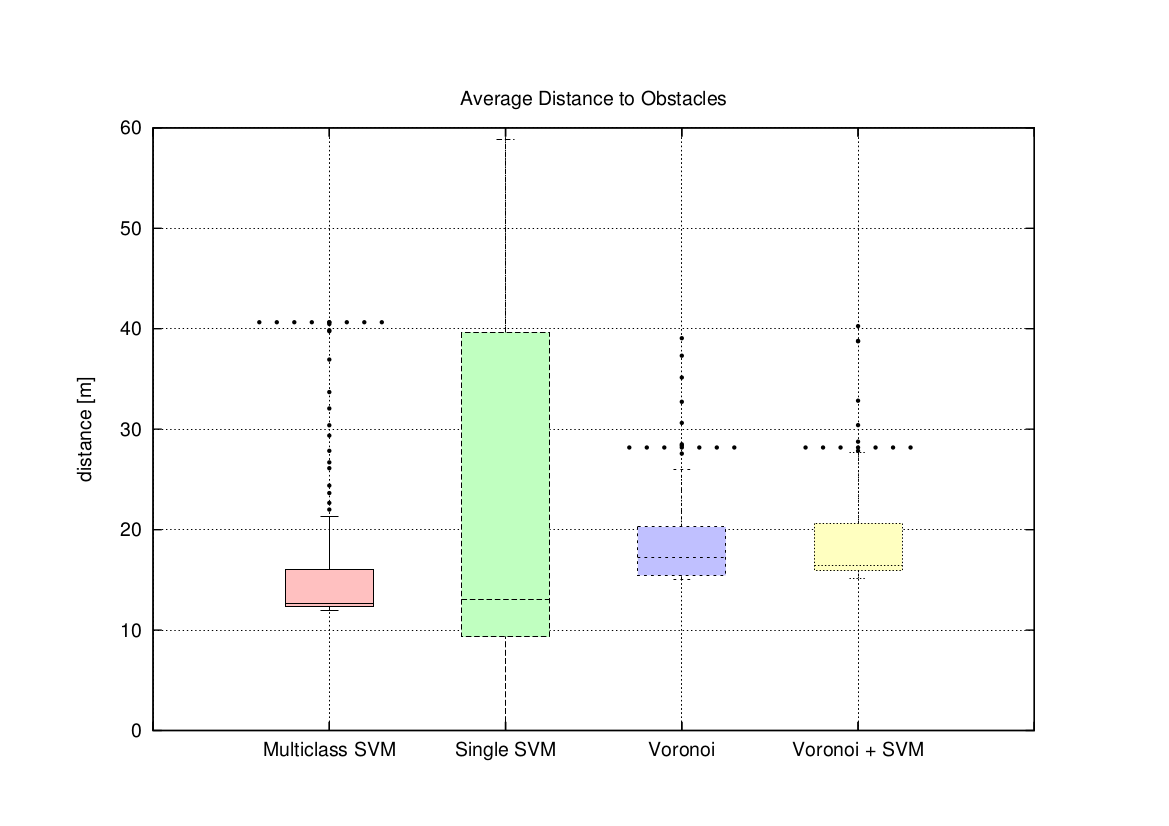
\includegraphics[width=\textwidth, trim=55 50 85 60,clip]{figure11}
	  \caption{Average distance to obstacles.}
	  \label{fig:cp06_avg_dist_all}
  \end{subfigure}  

  \begin{subfigure}[b]{\textwidth}
	  \centering
	  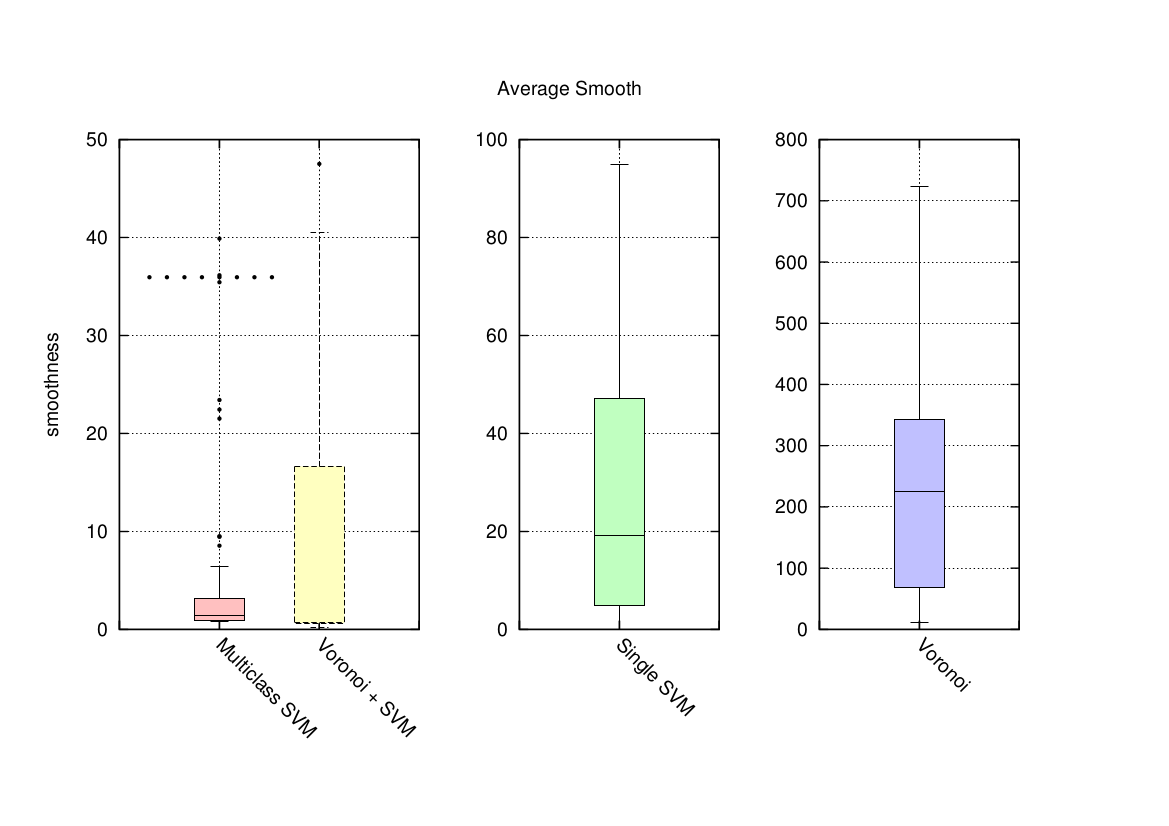
\includegraphics[width=\textwidth, trim=55 50 85 60,clip]{figure12}
	  \caption{Smoothness.}
	  \label{fig:cp06_smoothness_all}
  \end{subfigure}        
\phantomcaption % new inserted command
\end{figure*}

\begin{figure*}
  \ContinuedFloat
  \begin{subfigure}[b]{\textwidth}
	  \centering
	  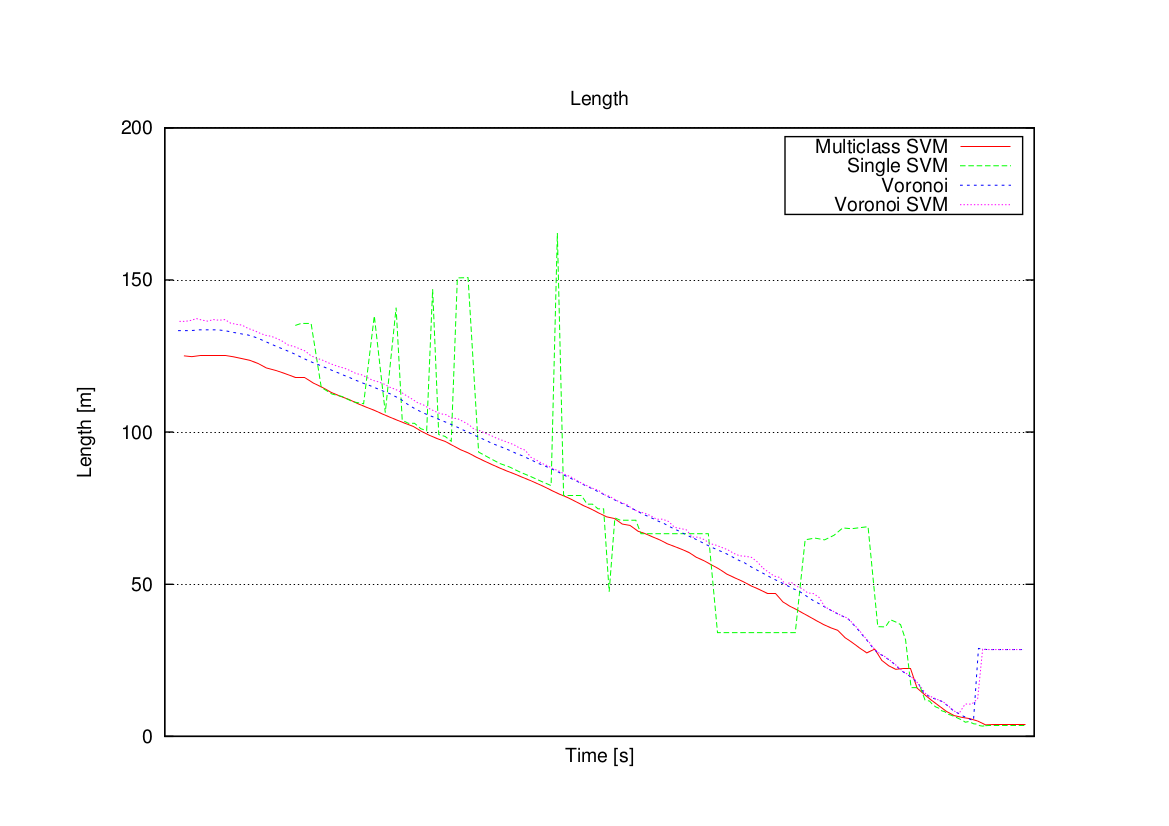
\includegraphics[width=\textwidth, trim=55 50 85 60,clip]{figure13}
	  \caption{Length.}
	  \label{fig:cp06_length_all}
  \end{subfigure}
  
  \caption{Results obtained after the comparison of the different methods.}\label{fig:cp06_results_comparison}
\end{figure*}

\subsubsection{Average distance to obstacles}\label{ch:chapter06_02_02_01}

In the chart of the figure \ref{fig:cp06_avg_dist_all}, we can see how the worst results were obtained by the \textit{Single \ac{SVM}} method. This method shows also a big variance in its results. This is due to the fact that results depend on the patterns analyzed, as well as the fact that using a single \ac{SVM} for a lot of obstacles with hidden corners, curves, etc. can give an unpredictable result. It is easy to deal with these difficulties if you separate the obstacles, as done with our method, or as done by \textit{Voronoi}, which shows a good behavior in this measure. In fact, results obtained by \textit{Voronoi} are better than those shown by our method, but this is because \textit{Voronoi} diagram always find the central point between each pair of points. However, as shown later, in other tests, this will become a disadvantage as it does not take into account other variables, like smoothness or length. Same applies to \textit{Voronoi+\ac{SVM}}, which shows a good behavior, as it takes as base the path given by the \textit{Voronoi} method.
Our method, despite of not having so good results, presents a good average distance to the obstacles, with an acceptable variance.

\subsubsection{Smoothness}\label{ch:chapter06_02_02_02}

As shown in the charts in figure \ref{fig:cp06_smoothness_all}, our method completely outperforms the results obtained by \textit{Single \ac{SVM}} and \textit{Voronoi}, as they are in a scale completely bigger than ours. Regarding to \textit{Voronoi+\ac{SVM}} method, it is not so bad if compared to the other two methods, but the measured smoothness is not as good as that measured for our method, which is much smaller and with a smaller variance, too.

\subsubsection{Length}\label{ch:chapter06_02_02_03}

About length, figure \ref{fig:cp06_length_all} shows the evolution of the path lengths for the four analyzed methods. The peaks of the \textit{Single \ac{SVM}} method stand out. These are due to the change in the patterns, so depending on the random pattern finally chosen, the path could change, avoiding the obstacles by their right or left randomly, producing changes in the measured length, as can be appreciated in the chart. This effect can be seen better in the videos. Also, it is possible to see that there are not results until a few iterations later than the other methods, due to the fact that in the conditions existing in these instants, the method was unable to find a feasible path.

Both \textit{Voronoi} and \textit{Voronoi+\ac{SVM}} methods reduce their length monotonically as expected except at the end of the route because the vehicle is too near to the goal and the diagram generated by Voronoi makes the car doing a turn. Despite of this particular effect, results of both methods are good, but not as good as those shown by our method, which always find a shortest path, because unlike Voronoi does, our method is able to avoid doing extra turns when finding the path by approaching a little more to the obstacles, when possible. This allows finding shorter and smoother paths, which are distant enough to the obstacles, but is the reason for which average distance to obstacle is slightly lower in our method.

As a final comparison, at figure \ref{fig:cp06_final_path_comparison} we can see the path obtained for each planner given the same position and goal. As can be seen, \textit{Multiclass \ac{SVM}} is the smoother of all them, showing also a safe path, which is far enough from the obstacles.

\begin{figure*}[h!]
  \centering
  \begin{subfigure}[b]{0.45\textwidth}
	  \centering
	  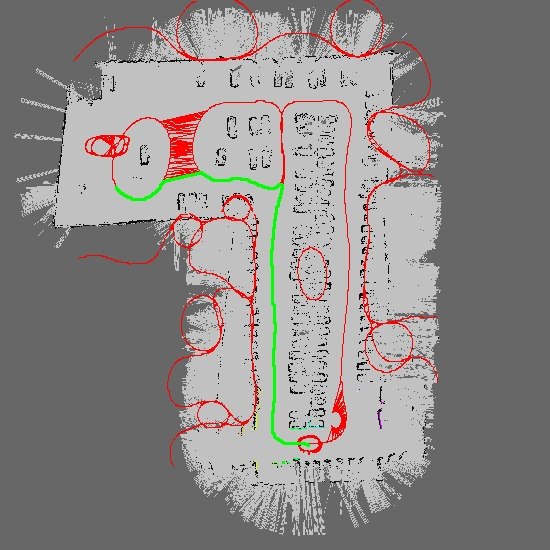
\includegraphics[width=\textwidth, trim=0 0 0 0,clip]{figure14}
	  \caption{Multiclass \ac{SVM}.}
	  \label{fig:cp06_multi_svm_final}
  \end{subfigure}%        
  ~
  \begin{subfigure}[b]{0.45\textwidth}
	  \centering
	  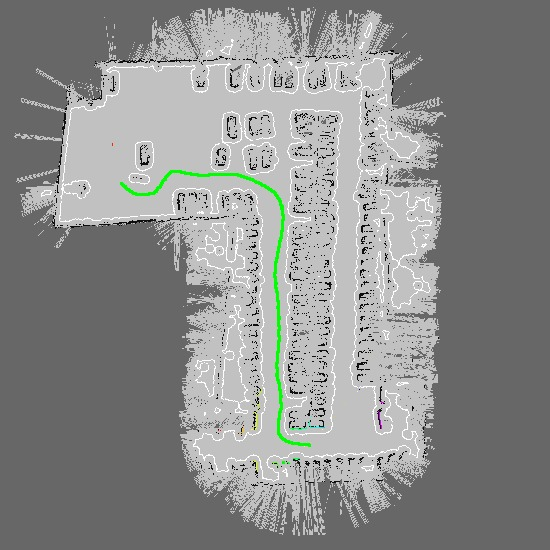
\includegraphics[width=\textwidth, trim=0 0 0 0,clip]{figure15}
	  \caption{Single \ac{SVM}.}
	  \label{fig:cp06_singl_svm_final}
  \end{subfigure}
  ~
  \begin{subfigure}[b]{0.45\textwidth}
	  \centering
	  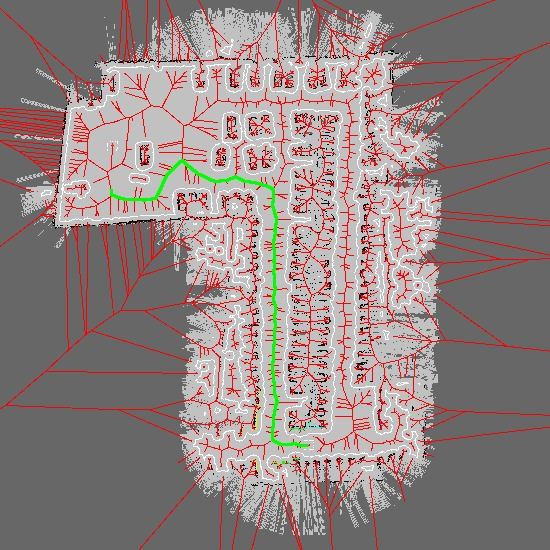
\includegraphics[width=\textwidth, trim=0 0 0 0,clip]{figure16}
	  \caption{Voronoi.}
	  \label{fig:cp06_voronoi_final}
  \end{subfigure}%
  ~
  \begin{subfigure}[b]{0.45\textwidth}
	  \centering
	  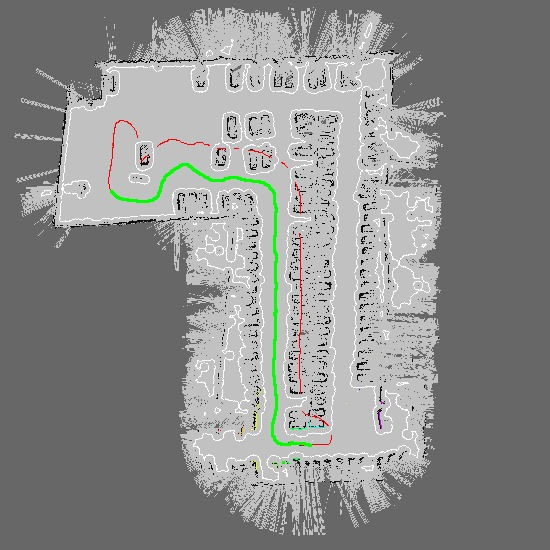
\includegraphics[width=\textwidth, trim=0 0 0 0,clip]{figure17}
	  \caption{Voronoi + \ac{SVM}.}
	  \label{fig:cp06_voronoi_svm_final}
  \end{subfigure}
  \caption{Final path obtained for the four methods compared.}\label{fig:cp06_final_path_comparison}
\end{figure*}

\section{Summary}\label{ch:chapter06_03}

In this chapter, we have shown an alternative to classical path planning methods, based on a \acf{MSVM}. Advantages of using this method as a base for our algorithm is that we can generate continuous non-linear separating surfaces between classes that, joined all together, allow the creation of a graph used for the generation of smooth, short and safe paths.
The method has been developed taking advantage of the use of a \ac{GPU} in order to reduce the required computational time, being able to work in real time applications. 

In this method, we have considered an initial graph, which is extended in the following iterations, allowing the inclusion of the new obstacles and the influence of the vehicle itself in the generation of the trajectories. In the next chapter, we will see a method able to follow the trajectories generated by this or another method.